\section{Gerarchia dei processi}
I sistemi UNIX/Linux prevedono che all' avvio del sistema entri in esecuzione il processo \emph{init}, che è mandato in esecuzione dal kernel durante il boot ed ha PID 1.
Tutti gli altri processi che il nostro sistema ospita discendono da init, ed i figli di qualsiasi processo che muore vengono adottati da questo processo init.

In Debain/Ubuntu l' init system è \emph{systemd}.
Per vedere l' albero dei processi possiamo utilizzare il comando \verb{pstree{.

\subsection{Gruppi di processi}
I processi sono organizzai in gruppi.
Quando viene mandato in esecuzione un nuovo processo, a questo viene associato un nuovo process group.
Se questo processo genera dei figli i figli appartengono allo stesso gruppo del padre e viene preservato anche in caso di \verb{exec{.

I gruppi permettono di mandare segnali ad una gerarchia di processi e sono alla base del \emph{job-control} offerto dalla shell.

\subsection{Identificatori di un processo}
In definitiva un processo ha vari identificatori:
\begin{itemize}
    \item PID: ID univoco del processo
    \item PPID: ID del processo padre
    \item PGID: id del process group a cui appartiene il processo
    \item RUID: Real user ID, indica l' id dell' utente/gruppo che ha mandato in esecuzione il processo
    \item RGID: Real group ID, indica l' id del gruppo primario dell' utente che ha mandato in esecuzione il processo
    \item EUID, EGID: Effective user/group ID, differiscono dal RUID/RGID se il comando che è stato eseguito ha il bit SUID/SGID attivo
\end{itemize}
Un processo utente può inviare segnali ad un altro processo solo se il suo EUID/RUID coincide con il RUID del processo destinatario, quindi possiamo inviare un segnale ad un processo solo se questi processi sono stati lanciati dagli stessi utenti o se il programma che invia il segnale è stato lanciato con un SUID uguale all' utente che ha spawnato il processo che riceve il segnale.

Es:
\begin{figure}[H]
    \centering
    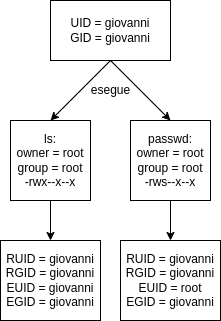
\includegraphics[width=125px]{images/3L_Gerarchia_di_processi/ruid_rgid_euid_egid.png}
\end{figure}
NB: si ricordi che questi ID in realtà sono numerici ma per capirci meglio usiamo il nome associato a loro.


Abbiamo a disposizione una serie di system call per ottenere queste informazioni:
\begin{verbatim}
    pid_t getpid()
        // Restituisce il PID
    
    pid_t getppid()
        // Restituisce il PID del padre
    
    pid_t getpgrp()
        // Restituisce il process group di chi la chiama
    
    uid_t getuid()
        // Restituisce lo user ID
    
    uid_t getgid()
        // Restituisce il group ID

    uid_t geteuid()
        // Restituisce l' effective user ID

    uid_t getegid()
        // Restituisce l' effective group ID
\end{verbatim}
Esistono anche alcune primitive per settare qualcuno di questi parametri ma possiamo farlo solo per andare verso privilegi minori, per esempio:
\begin{verbatim}
    int seteuid(uid_t)
        // Setta l' effective user id a quello passato
        // se possibile
    ...
\end{verbatim}

\subsection{Priorità dei processi}
Lo scheduler Linux assegna la CPU ai processi tenendo conto di un livello di priorità assegnato a ciascun processo e dipende principalmente dalla classe di scheduling del processo (real-time o normale).

La priorità dei processi normali può essere in parte controllata mediante il concetto di \emph{niceness} e la relativa system call \verb{nice{.
Più è alto il valore della niceness e più è bassa la priorità del processo.
Ogni processo ha un valore nell' intervallo [-20, 19] e di default è 0.
Un utente normale può solo aumentare la niceness di un suo processo, per abbassarla deve farlo fare per forza all' utente root.

Per lanciare un programma con un certo valore di niceness possiamo usare:
\begin{verbatim}
    nice -n <valore> comando
\end{verbatim}

Possiamo altresì modificare la niceness di un processo già in esecuzione con:
\begin{verbatim}
    renice <valore> PID
\end{verbatim}

\subsection{Job-control}
Il job-control permette di sospendere e riattivare gruppi di processi, questa funzionalità è offerta dalla shell mediante opportuni comandi.
La shell associa un job ID ad ogni comando eseguito, anche una pipeline di comandi ha un singolo job ID.
Per visualizzare i job attivi si può usare il comando \verb{jobs{.

Possiamo avere dei processi in foreground, quindi processi che hanno il controllo dello standard input, output ed error.
Di fatto prende il controllo del terminale e lo restituisce alla fine del processo.

Ma possiamo anche avere dei job in background, per fare ciò lancio il processo con la sintassi:
\begin{verbatim}
    comando &
\end{verbatim}
in questo modo il processo lanciato non ha accesso allo standard input (ma ha ancora accesso allo standard output ed error).
Quindi l' utente può tornare ad utilizzare la shell mentre il job viene completato.

Se abbiamo un processo in foreground e vogliamo stopparlo possiamo usare CTRL+Z (che equivale ad inviare il segnale SIGSTP), una volta fatto ciò possiamo intervenire sui job stoppati:
\begin{itemize}
    \item riavviarli in foreground:
\begin{verbatim}
    fg %JOB_ID
\end{verbatim}
    \item riavviarli in background:
\begin{verbatim}
    bg %JOB_ID
\end{verbatim}
    \item inviare un segnale:
\begin{verbatim}
    kill %JOB_ID
        # invia SIGTERM
    kill -n SIGNAL %JOB
        # invia il segnale SIG
\end{verbatim}
\end{itemize}

Se il terminale viene chiuso i job in esecuzione ricevono il segnale SIGHUP e di default vengono terminati.
Per fare si che i job non vengano chiusi all' uscita dal terminale possiamo usare:
\begin{itemize}
    \item 
\begin{verbatim}
    nohup comando
\end{verbatim}
    il job eseguito sarà immune a SIGHUP, non avrà accesso allo stdin, quindi se dovesse leggere riceverebbe EOF.
    Mentre l'output viene rediretto verso il file \verb{nohup.out{
    \item
\begin{verbatim}
    disown %JOB_ID
\end{verbatim}
    rende immune a SIGHUP un job già in esecuzione.
    Il job viene quindi rimosso dalla tabella dei job, in questo modo alla chiusura la shell non invierà SIGHUP.
    Il processo non avrà accesso allo standard input e si dovrà redirezionare l' output su un file manualmente.
\end{itemize}

\subsubsection{top}
Il comando top ci permette di visualizzare i processi ed effettuare operazioni su di essi in modo interattivo.
I processi sono ordinati per utilizzo decrescente della CPU, possiamo inviare segnali ai processi e cambiarne la niceness.
Ci vengono mostrate anche informazioni aggiuntive sull' intero sistema come l' utilizzo della CPU, delle memorie, ecc.
Alcuni comandi che possiamo dare sono:
\begin{itemize}
    \item \verb{h{ : per ottenere aiuto
    \item \verb{d{ : per settare l' intervallo di aggiornamento
    \item \verb{k{ : per inviare un segnale
    \item \verb{n{ : per settare il numero di processi da visualizzare
    \item \verb{r{ : per modificare la niceness
    \item \verb{u{ : per settare l' utente da visualizzare
    \item \verb{q{ : per uscire
\end{itemize}
